El enfoque de la aplicación en ensamblador era poder procesar la mayor cantidad de pixeles contiguos (16 bytes) con instrucciones SIMD para poder aprovechar al máximo el paralelismo que estas ofrecen. Esto no fue posible debido a que el set de instrucciones no tiene comparaciones de greater, lower o derivadas para bytes sin signo (necesario ya que los pixeles en grayscale van del 0 al 255) por lo que fue necesario realizar un desempaquetamiento de los datos (convirtiendolos en words) para luego hacer las comparaciones correspondientes.

Para optimizar el procesamiento dentro del ciclo, se calcula y se guarda en registros xmm al inicio del programa:
\begin{itemize}
  \item xmm12 $\Rightarrow$ Contiene 16 bytes packed con el mínimo
  \item xmm11 $\Rightarrow$ Contiene el mínimo packed en words
  \item xmm5 $\Rightarrow$ Contiene el máximo packed en words
  \item xmm6 $\Rightarrow$ Contiene la representación flotante de Q packed
\end{itemize}

También se calcula y se guarda en el registro rcx, la cantidad de pixeles que tiene la imagen, información que se utilizará para conocer cuántos pixeles faltan por procesar en cada iteración.

\subsubsection{Descripción del ciclo}
Al comienzo del ciclo se ponen en 0 los bytes del registro xmm8 que servirá como acumulador de los nuevos valores que tendrán los pixeles.

Se guardan 16 bytes contiguos desde la imagen fuente en el registro xmm1, se busca cuáles son iguales al mínimo (aprovechando la instrucción pcmpeqb que realiza la comparación en los 16 bytes simultaneamente) y se guarda la máscara obtenida que se usará mas tarde. Luego se los desempaqueta en parte alta y baja extendiendolos a words para realizar comparaciones.

\begin{figure}[H]
\centering
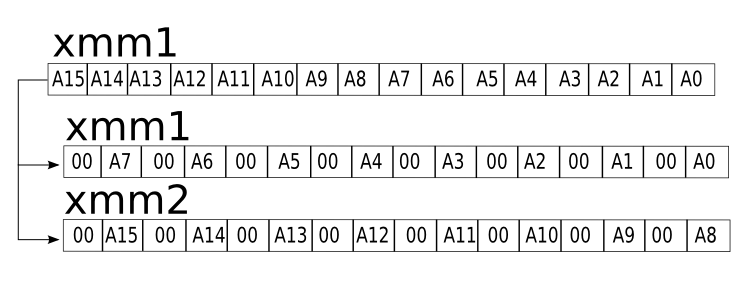
\includegraphics[width=90mm]{unpackxmm1.png}
\caption{Desempaquetado de los bytes a words para realizar comparaciones}
\label{overflow}
\end{figure}

Se buscan los números que superen al máximo comparando la parte alta y baja con el registro xmm5 preparado al inicio del programa el cuál contiene el máximo en words empaquetadas. Utilizando pcmpgtw tanto en la parte baja como la alta, obtenemos una máscara que contiene en 0xFFFF las words mayores al máximo y en 0x0000 las demás. Empaquetamos la máscara relacionada a la parte baja y a la alta dejando en 255 sólo los bytes que sean mayores al máximo para luego sumarlos en el acumulador.


\begin{figure}[H]
\centering
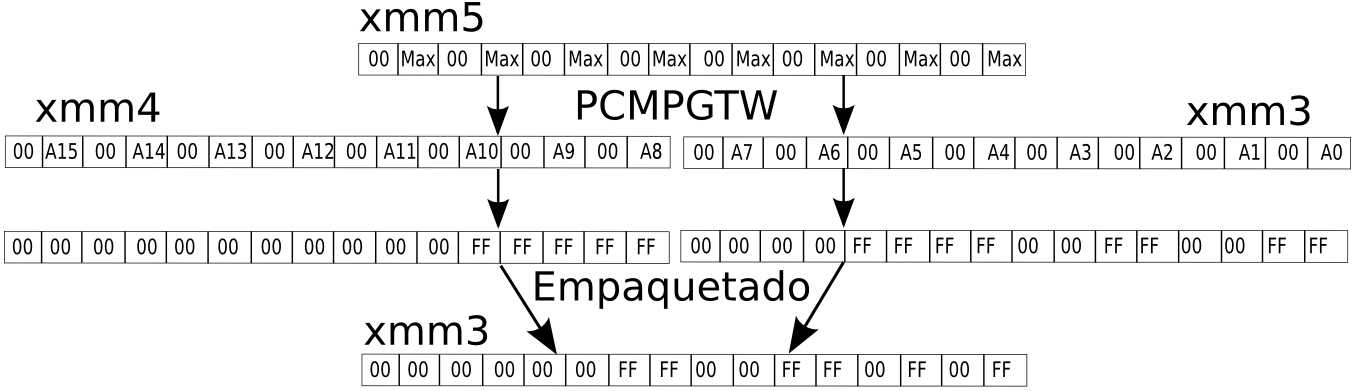
\includegraphics[width=150mm, height=40mm]{cpmmax.png}
\caption{Ejemplo de creación de máscara y empaquetado de la misma. El registro xmm3 es la copia de xmm1 que guardará la parte baja de la máscara, xmm4 realiza lo mismo con la parte alta.}
\label{overflow}
\end{figure}

Al utilizar un acumulador incialmente en 0 se pudo ahorrar el paso de comparar los pixeles menores al mínimo ya que los pixeles que cumplieran esta propiedad tendrían 0 como valor.

Para conseguir la máscara para el caso en el que el valor del pixel estuviera entre el máximo y el mínimo ($min \geq pixel \leq max$) se aprovechó las máscaras previamente obtenidas (mayores al máximo e iguales al mínimo), por lo que sólo fue necesario buscar los números mayores al mínimo (haciendo un procedimiento similar al de la búsqueda del máximo), agregarle los números iguales al mínimo (mediante un por) con la máscara creada al principio del ciclo y luego sacarle los mayores al máximo (mediante un pxor).

Luego de haber creado la máscara para el caso, se realiza el cálculo de los nuevos valores para los pixeles que cumplan esa propiedad, los cuales deben realizarse utilizandose punto flotante. Fue necesario desempaquetar aún más los pixeles para poder obtener los valores de estos en double words y poder convertirlos a single precision floats, precisión suficiente para los cálculos que también brinda la posibilidad realizar más operaciones sobre los pixeles simultanteamente que con doubles.

Se realiza el desempaquetado de la parte baja anteriormente desempaquetada (xmm1) y se los convierte a single presicion floats. Luego se los divide por el registro xmm6 el cuál contiene el valor Q empaquetado en single presicion floats calculado al inicio del programa. Se lo trunca para realizar la función "floor" convirtiendose en entero, se lo convierte otra vez a float y se lo termina multiplicando por xmm6 otra vez para finalmente ser convertido a entero, obteniendo el valor correspondiente para cáda pixel. Se vuelve a empaquetar obteniendose otra vez los valores nuevos de los pixeles en words y se repite la operación con la parte alta del desempaquetamiento inicial (xmm2).

\begin{figure}[H]
\centering
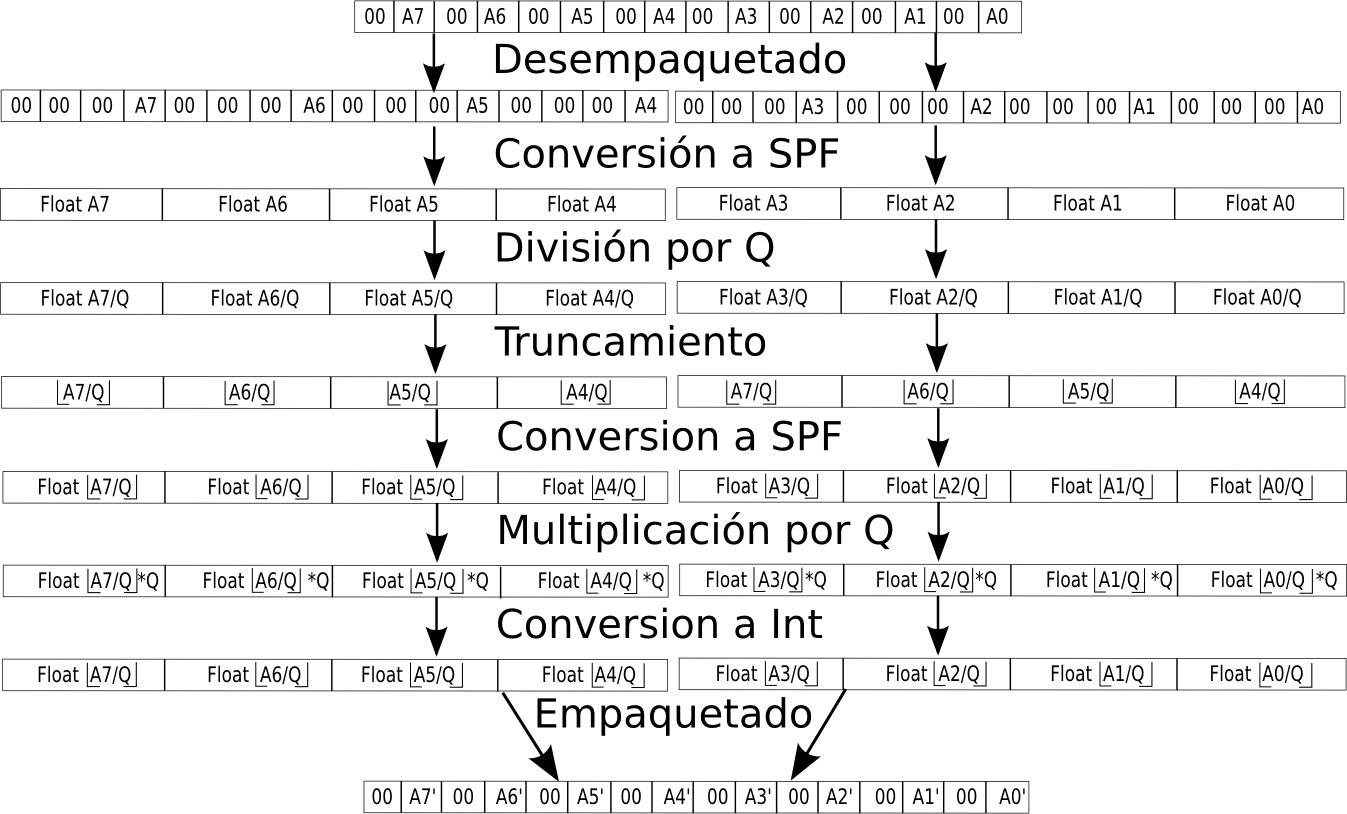
\includegraphics[width=150mm, height=85mm]{calcq.png}
\caption{Ejemplo del cálculo de la parte baja de los nuevos valores para los pixeles que entran en el caso ($min \geq pixel \leq max$), el mismo procedimiento se realiza con la parte alta y se empaquetan ambos resultados}
\label{overflow}
\end{figure}

Al finalizar, se empaquetan los dos registros resultantes para luego poder aplicarle la máscara anteriormente creada para el caso y sumar el valor obtenido al acumulador, dejando el valor correspondiente en los pixeles que cumplían con el caso.

Por último, se copian los nuevos valores de los 16 bytes en la imagen destino, se incrementan los punteros de la imágen fuente y destino para la próxima iteración. También se resta nuestro contador de pixeles, se lo compara para ver si llegó al final, caso en el que termina la ejecución, o si quedan más e igual, caso en el que vuelve a ciclar, o si restan menos de 16 bytes por agarrar, dónde se vuelve para atrás los punteros de las imágenes para que queden 16 pixeles exactamente y se pueda realizar la última iteración.

\subsubsection{Comparación con el lenguaje C}
Enfocandonos en la versión decompilada de umbralizar\_c.c utilizando objdump -d -M intel -S umbralizar\_c.o se pueden observar bien en detalle las instrucciones que utiliza el compilador para ensamblar la versión en c de umbralizar.

Se puede observar (Figura 4) que el compilador, al tratarse del lenguaje C y su convención utiliza el stack para guardar variables locales, algo que seguramente será cubierto por la memoria caché pero que es comparable contra utilizar casi únicamente registros, que otorgan mejor performance a la hora de utilizar datos, como se realiza en la implementación en ensamblador.
\begin{lstlisting}
if(src_matrix[y][x] < min) {

;Instrucciones para settear la posicion del byte
mov    eax,DWORD PTR [rbp-0x4c]
movsxd rdx,eax
movsxd rax,ebx
imul   rdx,rax
mov    rax,QWORD PTR [rbp-0x38]
add    rdx,rax
mov    eax,DWORD PTR [rbp-0x48]
cdqe   
movzx  eax,BYTE PTR [rdx+rax*1]
;Termina el setteado de la posicion del byte
cmp    al,BYTE PTR [rbp-0x70] ;Realiza la comparacion
jae    c3 <umbralizar_c+0xc3>

dst_matrix[y][x] = 0;

;Instrucciones para settear la posicion del byte
mov    eax,DWORD PTR [rbp-0x4c]
movsxd rdx,eax
movsxd rax,r12d
imul   rdx,rax
mov    rax,QWORD PTR [rbp-0x28]
add    rdx,rax
mov    eax,DWORD PTR [rbp-0x48]
cdqe   
;Termina el setteado de la posicion del byte
mov    BYTE PTR [rdx+rax*1],0x0 ;Pone en un pixel de la imagen fuente 0x0
jmp    171 <umbralizar_c+0x171>
\end{lstlisting}

Figura 4: Comparación y asignación de valor a un pixel utilizando el código  ensamblador generado para el código C por gcc. \\

Enfocandonos en los condicionales, parte importante del código ya que estos les darán el valor nuevo a cada pixel, se puede ver como la versión en C desensamblada produce el código respectivo para calcular la posición del byte específico a comparar en la matríz fuente cada vez que se quiere llamar a un pixel (dst\_matrix[y][x]) (Figura 4). La diferencia en eficiencia en esta implementación en C contra la versión en ensamblador es muy evidente, no sólo no es necesario calcular la posición ya que se toman 16 bytes contiguos en vez de la utilización del casteo matricial, si no que las comparaciones o el cálculo de nuevos valores se realizan en simultaneo. Si bien el código en c podría cambiarse para hacer un recorrido lineal tal cómo lo hace ensamblador, la implementación en ensamblador nos otorga la capacidad de poder ser detallistas a la hora de la utilización de recursos y en este caso, usar instrucciones SIMD.

Debe notarse que en la versión en assmembler, debido a la utilización de instrucciones SIMD se comparan y se procesan 8 bytes por instrucción (excepto en el caso de cálculo de punto flotante) y 16 bytes por cada ciclo del algoritmo. Al hablar de procesar, se tienen en cuenta las operaciones tanto de comparación como de cálculo para los valores resultantes de los píxeles. También queda en evidencia que el algoritmo programado en assembler hace sólo dos llamadas a memoria, una para traer los 16 bytes contiguos y otra para poner en la imagen de destino estos 16 bytes con sus nuevos valores, lo que es más eficiente que acceder a memoria de a byte como lo hace la implementación en c en cada iteración.

Para el caso del cálculo de los nuevos valores para los pixeles ($min \geq pixel \leq max$) en dónde se utilizó punto flotante para calcular $\lfloor pixel/q \rfloor * q$, las operaciones de punto flotante se realizan en la versión en assembler con 4 pixeles por instrucción SIMD, incrementando también la eficiencia contra la versión en c en la cuál se hace el cálculo de un sólo píxel por instrucción.